\section{Agile Methoden und Open Source}
(Autor: Henn)\\

Der große Hype um agile Methoden ist bereits vorüber. Doch haben agile Methoden die herkömmliche Softwareentwicklung nachhaltig beeinflusst. Die Fachzeitschriften sind voll davon und in Firmen werden agile Vorgehensweisen immer häufiger umgesetzt. Doch wie sieht die Situation in Open Source Projekten mit ganz anderen Umständen und Herausforderungen aus?

In diesem Abschnitt wird ein Blick in die Open Source Welt geworfen und
analysiert, inwiefern agile Techniken eingesetzt werden. Im Anschluss werden
Chancen und Probleme bei der Verwendung eines agilen Modells im Open Source
Bereich dargestellt.


\subsection{Open Source Projekte}
Bei der Recherche viel auf, dass es gar nicht so leicht ist, Open Source
Projekte zu finden, die von sich selbst behaupten, sie würden nach agilen
Vorgehensmodellen vorgehen. Allerdings finden sich auch in normalen Projekten
Techniken, die eindeutig aus der agilen Softwareentwicklung stammen. Im Folgenden
sollen einige Projekte als Stellvertreter für die verschiedenen Stufen der
Adaption mit Blick auf die Umsetzung agiler Techniken und Prinzipien betrachtet werden.

\subsubsection{TYPO3}
Die Entwickler des Open Source Content Management Systems TYPO3 haben sich dazu
entschieden, ihre nächste Version 5 (Phoenix) vollständig nach dem Scrum Vorgehensmodell zu
entwickeln. Anhand dieses Beispiels soll gezeigt werden, wie es möglich ist,
ein solches Vorgehensmodell im Open Source Bereich vollständig umzusetzen und
was es für Bedingungen gibt, damit dies erfolgreich geschehen kann.
\begin{figure}[h]
	\centering
	
\includegraphics[width=1\textwidth]{images/typo3_Phoenix_logo.jpg}
	\caption{Logo TYPO3 5.0 Phoenix}
	\label{Logo-Phoenix}
\end{figure}

Ein Sprint dauert beim TYPO3 Phoenix Team 4 Wochen. Innerhalb dieses Sprints finden tägliche
Meetings statt und am Ende eines Sprints muss eine lauffähige Version bereit stehen. Abbildung 
\ref{magic-cycle} visualisiert diesen Zyklus. User Stories aus dem Product Backlog werden für
diesen Sprint ausgesucht und in einem Sprint Backlog festgehalten. Diese Stories werden dann
innerhalb der 2-4 Wochen implementiert.
\begin{figure}[h]
	\centering
	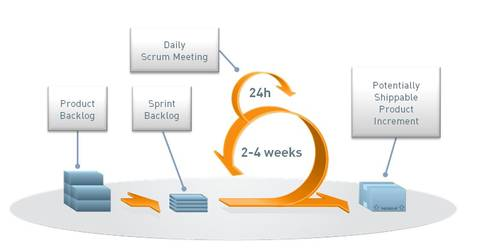
\includegraphics[width=1\textwidth]{images/typo3-magic-cycle.jpg}
	\caption{Magic Cycle - TYPO3 Scrum Implementierung}
	\label{magic-cycle}
\end{figure}


Als Product-Owner, der in Firmen in der Regel aus einer Person besteht, wurde für TYPO3
ebenfalls ein kleines Team bestehend aus drei Personen eingerichtet. Dies erscheint sinnvoll, da es
sich bei TYPO3 ja um eine Gemeinschaftsentwicklung handelt. Eine einzelne Person als Product-Owner
würde dem Community Gedanken entgegen wirken und  wäre darüber hinaus Person wahrscheinlich auch
noch überlastet, wenn sie plant, diese Aufgabe in ihrer Freizeit auszufüllen. Diese drei
Personen diskutieren über die Features, die innerhalb eines Sprints implementiert werden sollen
und priorisieren diese.
\newline Die Rolle des Scrum-Masters wird wiederum nur von einer Person besetzt. Auch dies ergibt
durchaus Sinn, da sich zwei Scrum-Master, oder sogar ein Team von Scrum-Masters eher gegenseitig bei
der Leitung von Gesprächen behindern würde.
\newline Das eigentliche Scrum-Team für die TYPO3 Entwicklung besteht aus 19 Entwicklern. Die alle
miteinander in Kontakt stehen und koordiniert werden müssen. Entscheidend für den Erfolg von Scrum
ist daher das Internet. Es bietet vielfältige Möglichkeiten, miteinander zu kommunizieren und große
räumliche Entfernungen zu überbrücken. So kommuniziert das Team:
\begin{itemize}
\item Sprint-Planung, Review und Retrospektive werden durch Meetings im Internet durchgeführt.
\item Es steht ein Jabber Chatroom bereit, in dem sich das Team kurzfristig abstimmen kann und
Fragen während der Entwicklung geklärt werden.
\item jeden Tag findet um 17:00 Uhr das Daily Scrum Meeting mittels Webex oder Skype statt. Danach
wird das Protokoll der Sitzung über die Mailing Liste verschickt, damit alle, die nicht teilnehmen
konnten, trotzdem auf dem neusten Stand sind.
\item Das Sprint-Backlog wird ebenfalls im Internet unter forge.typo3.org gepflegt.
\item TYPO3 Veranstaltungen werden so oft, wie möglich genutzt um persönlich miteinander sprechen zu
können
\item Nach jedem Sprint wird das Ergebnis sowohl als Nachricht, als auch als laufende
Demo-Installation bekanntgegeben
\end{itemize}
\begin{figure}[h]
	\centering
	\fbox{
		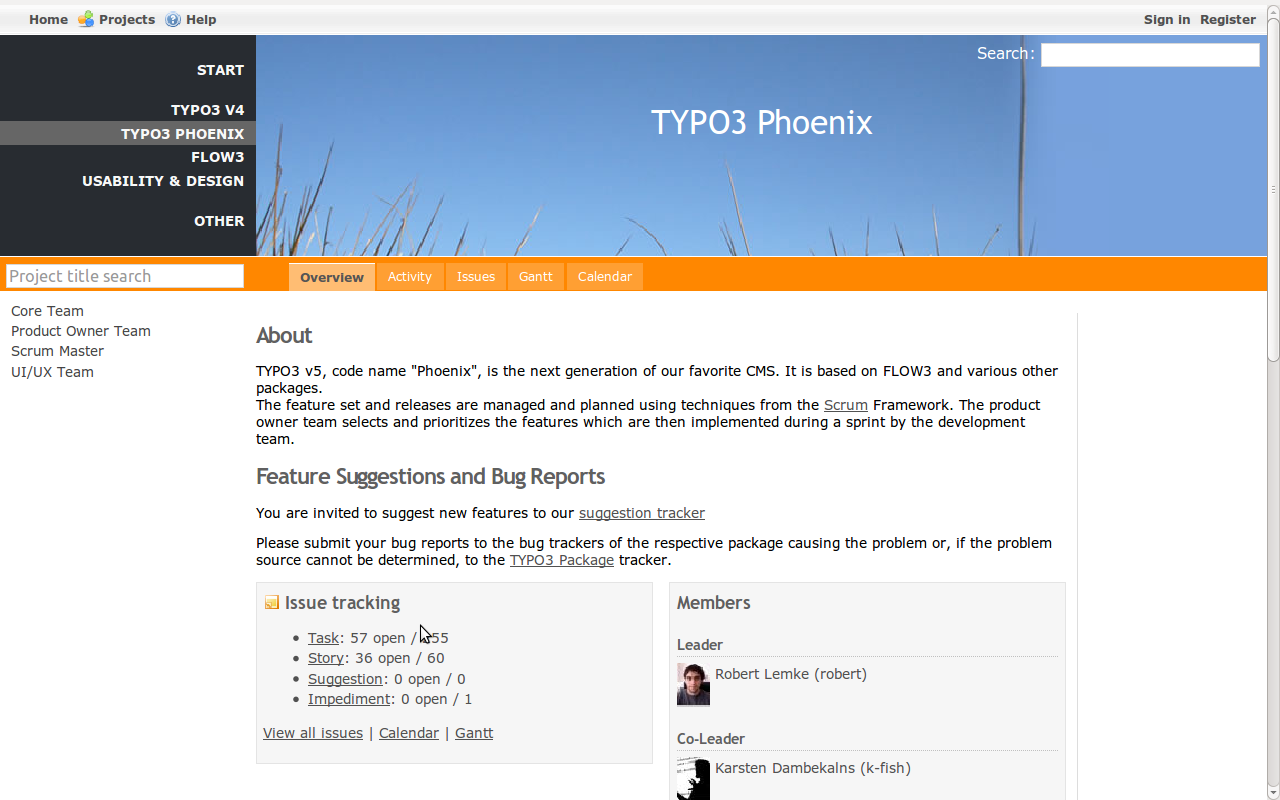
\includegraphics[width=1\textwidth]{images/forge-typo3-org.png}
	}
	\caption{forge.typo3.org}
	\label{forge}
\end{figure}
Der gesamte Fortschritt sowie die offizielle Dokumentation und Kommunikation wird über
die Web-Plattform forge.typo3.org dargestellt. Auf diese Weise ist der Entwicklungsprozess sehr
transparent und für die Community einsehbar. Dadurch verliert die Entwicklung nicht an Akzeptanz und
die freiwilligen Committer wissen, was gerade benötigt wird.

Auf der Website des Phoenix Teams wurden mehrere Bereiche eingerichtet:
\begin{description}
\item [Core Team] Hier befinden sich alle Informationen, die das Entwicklungs-Team zur Koordination
benötigt. der Bereich beinhaltet
\begin{itemize}
\item eine Übersicht mit Link zum Issue-Tracker und einer Liste der Team Mitglieder
\item Eine Auflistung aller bisher ausgeführten Aktivitäten, wie Wiki Änderungen, oder auch
Änderungen am Quellcode
\item Eine Roadmap für den aktuellen Sprint, mit Auflistung aller in diesem Sprint zu erledigenden
User Stories und den dazugehörigen Tasks
\item den Issue Tracker
\item das Sprint, sowie das Product Backlog
\item ein Gantt Chart
\item ein Kalender
\item  ein Wiki
\item das Repository mit dem Quellcode
\end{itemize}
Das Wiki beinhaltet alle wichtigen Informationen für Entwickler, sowie teilweise Erklärungen zum
Scrum Prozess und Richtlinien.  So findet sich dort zum Beispiel die Erklärung, was es mit der
''Definition of Done``  auf sich hat, die bei Scrum ein wichtiges Artefakt darstellt.
\item [Product Owner Team] Für das Product Owner Team gibt es ebenfalls wie beim Core Team eine
Übersicht mit den Mitgliedern, sowie eine kurze Beschreibung der Gründe, sich für ein Teams als
Product Owner zu entscheiden. Es finden sich ebenso Übersichten über Aktivitäten, Issues und
Termine. Außerdem wird ebenfalls ein Wiki gepflegt. Dieses Wiki behandelt  allerdings viel
stärker den Scrum Entwicklungsprozess, als das Wiki des Core Teams. So ist hier der eigentliche
Entwicklungsprozess für TYPO3 Phoenix beschrieben, sowie für alle, die Scrum noch nicht so intuitiv
leben ein kleines Cheat Sheet hinterlegt, das den Scrum Prozess nochmal auf einer Seite
übersichtlich zusammenfasst. Ebenso findet sich hier eine Liste mit Benutzerrollen für TYPO3. Im
Anschluss daran sind die Protokolle der einzelnen Scrum Meetings hinterlegt.
\item [Scrum Master] im Bereich des Scrum Masters gibt es lediglich eine Übersicht, einen Bereich
in dem die Aktivitäten aufgelistet werden, sowie Issue Tracker, Gantt Chart und ein Kalender. Da
die Rolle des Scrum Masters nur mit einer Person besetzt ist, muss hier auch nicht mehr Inhalt
bereit stehen.
\item [UI/UX Team] dieses Team beschäftigt sich mit dem User Interface, sowie der User Experience.
Es finden sich die Übersichten, über Issues und Aktivitäten, wie in den anderen Bereichen. 
\end{description}

Die TYPO3 Entwickler haben es geschafft, den gesamten Scrum Prozess mit minimalen Anpassungen
für ihr Projekt zu Adaptieren. Von entscheidendem Vorteil für die TYPO3 Entwickler, ist die
Tatsache, dass sie alle aus Deutschland kommen. So ist es deutlich einfacher, einen Termin, der auf
17:00 Uhr angesetzt wurde, auch wahrzunehmen. Eine solche regelmäßige zeitliche Abstimmung würde bei
Entwicklern, die über die ganze Welt verstreut sind nicht funktionieren. Außerdem ist es so für die
Projektteilnehmer leichter, zu den TYPO3 Veranstaltungen zu fahren, da diese ebenfalls hauptsächlich
in Deutschland stattfinden. Auch hier wäre es für einen weit verstreutes Entwicklerteam
auch finanziell nicht möglich, sich so oft persönlich zu sehen. Ein weiterer Faktor ist sicherlich
die Größe des Projektteams. Bei nur 17 Mitgliedern ist es leichter möglich,die Koordination über das Internet zu  organisieren und dafür zu sorgen, dass auch wirklich alle gerade aktiv am Projekt teilnehmen können.

\subsubsection{Firefox}
Das Firefox Projekt besteht aus zahlreichen Unterprojekten. Diese gehen teilweise sehr unterschiedlich vor.
\begin{figure}[h]
	\centering
	\fbox{
		
\includegraphics[width=0.5\textwidth]{images/firefox-3.jpg}
	}
	\caption{Logo Firefox}
	\label{fireLogo}
\end{figure}
So ist zum Beispiel das Tracemonkey Projekt, ein Just in Time (JIT) Compiler für JavaScript äußerst agil unterwegs. Das Projekt bezeichnet sich selbst als ''in rapid development mode''\cite{bib:trm}. So ist es zum Beispiel sehr leicht, Code beizutragen. Selbst wenn dieser nicht alle Tests bestanden hat. Man muss nur erklären, warum er den Test nicht besteht und was passieren muss, um diesen Fehler zu beheben'\cite{bib:trm}. Ein Vertreter der traditionellen Entwicklung ist zum Beispiel der Compositor, der  Teil der Rendering Engine Gecko ist \cite{bib:beltzner}

Mit der Version 4 des Firefox wurde ein neues Entwicklungsmodell eingeführt. Dies soll den Missstand beheben, dass es sehr lange dauert, bis einen neue Version des Firefox herausgegeben wird, die auch wirklich neue Features mit sich bringt. Ein Umstand, der die Motivation der Entwickler nicht gerade fördert, da neue von ihnen bereitgestellte Funktionen erst ein halbes bis dreiviertel Jahr später in einer Firefox Version zur Verfügung stehen. Außerdem ist der Firefox dadurch nicht so häufig in den Medien, wie andere Browser, die öfters neue Funktionalitäten bereitstellen.

Das Entwicklungsmodell soll die diversen Unterprojekte allerdings nicht in ihrem eigenen Entwicklungsmodell einschränken. Firefox Produkt Manager Mike Beltzner beschreibt dies wie folgt: ''Really, we're not tied to any specific development model, [...] We're tied to what is effective''\cite{bib:beltzner}. Nachfolgend soll dieses Entwickllungsmodell beschrieben werden und analysiert werden, inwieweit hier agile Prinzipien verfolgt werden.

Das neue Entwicklungsmodell sieht mehrere Entwicklungszweige vor, die pa\-ra\-llel geführt werden.
\begin{itemize}
\item mozilla-central
\item firefox-experimental (fx-exp)
\item firefox-beta (fx-beta)
\item Firefox
\end{itemize}
\begin{figure}[h]
	\centering
	\fbox{
		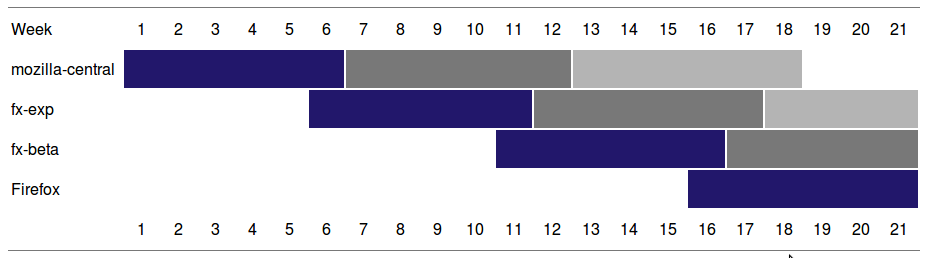
\includegraphics[width=1\textwidth]{images/timetable-firefox.png}
	}
	\caption{Zeitplan Firefox}
	\label{firett}
\end{figure}

Der Zweig mozilla-central stellt die Basis dar, in der die neusten Funktionalitäten entwickelt werden. jeweils im sechs Wochen Rhytmus werden diese Funktionalitäten, soweit sie reif genug sind in den nächst höheren Zweig überführt und dort weiter verbessert und stabilisiert, während im mozilla-central Zweig bereits an den nächsten Features gearbeitet wird. Dort besteht dann ebenfalls jeweils im sechs Wochen Rhythmus die Möglichkeit, neuen Code in den nächst höheren Zweig zu übertragen. So ist es theoretisch möglich, alle sechs Wochen eine neue Version des Firefox herauszugeben. Abbildung \ref{firett} zeigt den offiziellen Zeitplan des Firefox Projektes. der diesen sechs Wochen Rhythmus darstellt. Wie Abbildung \ref{fireusers} zeigt, stellen die verschiedenen Zweige außerdem eine neue Stufe im Testen dar. So wird sich die Zahl der Nutzer mit jedem Zweig verzehnfachen, um am Ende ein breit getestetes Produkt zur Verfügung stellen zu können.

Durch diese Umgestaltung ist es dem Firefox Team möglich, schnell neue Features in die offizielle Version zu bringen, ohne dass die einzelnen Unterprojekte dadurch ausgebremst werden. Teams, die traditionell entwickeln, können einfach mehrere Zyklen für sich in Anspruch nehmen und ihre Erweiterungen zu einem späteren Zeitpunkt in die nächst höheren Zweige überführen, Teams, die eher agil vorgehen werden diesen schnellen Release Zyklus nutzen und ihre neuste Version einbringen, ohne auf langsamere Projekte warten zu müssen.
\begin{figure}[h]
	\centering
	\fbox{
		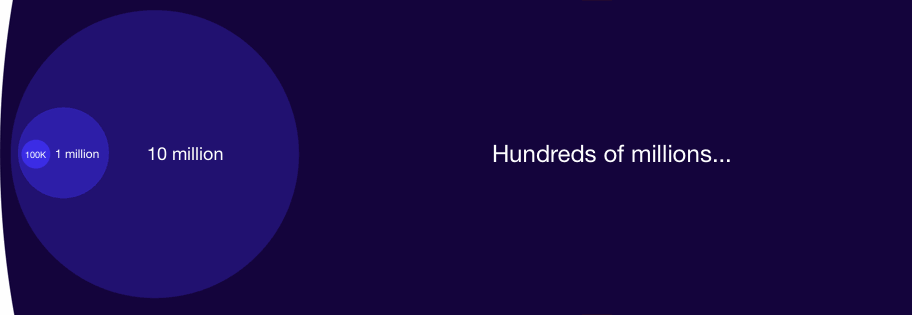
\includegraphics[width=1\textwidth]{images/firefox-channels-users.png}
	}
	\caption{Anzahl der Nutzer der in den verschiedenen Entwicklungszweigen}
	\label{fireusers}
\end{figure}


\subsection{Vorteile agiler Methoden in Open Source Projekten}
  - Motivation von Entwicklern und Community\\
  - Rasches Umsetzen neuer Anforderungswünsche\\
  - ...
  
\subsection{Nachteile agiler Methoden in Open Source Projekten}
  - Zeit\\
  - Ort\\
  - ...


